\documentclass[10pt,a4paper]{book}
\usepackage{graphicx, hyperref}
\graphicspath{{figures/}}

\title{A Laboratory Course on Single Molecule Localization Microscopy}

\author{Kyle M. Douglass}

\date{\today}

\begin{document}

\maketitle

\chapter{Introduction}

\section{Super-Resolution Fluorescence Microscopy}

Fluorescence microscopy is a set of techniques that allows scientists to study the structure and behavior of microscopic systems. Cell biologists in particular use fluorescence microscopes to visualize biological systems across many different spatial scales, from macromolecular complexes, organelles, and cells to tissues and even whole organisms. The power of fluorescence microscopy comes from the ability to label specific molecules with fluorescent markers such that the presence of light coincides with the presence of the target molecules. This molecular specificity, when combined with a light microscope's ability to magnify specimens that are normally too small to see with the unaided eye, provides a powerful tool to better understand the microscopic world.

All light microscopes, however, are bound by the laws of diffraction which state that the smallest features that can be observed by the instrument are approximately the size of the wavelength of light. Anything smaller than this so-called diffraction limit appears blurred, often to the point where an observer is completely unable to infer its structure from an image. For biologists this is particularly problematic because many important cellular structures have sizes that are smaller than this limit.

Starting in the 1900s researchers began to discover ways to circumvent the diffraction limit of light microscopy and image structures that were smaller than a wavelength with good fidelity. Among the first such techniques that was proposed and realized was the near-field optical microscope, whereby a sample is scanned by an illuminated aperture that is smaller than the wavelength of light. Unfortunately, this technique is somewhat cumbersome to use for cell biology studies because of the constraints that the instrument places on the sample. In the early 1990s it was discovered that the resolution of confocal fluorescence microscopes, a standard instrument in cell biology, could be improved beyond the diffraction limit by up to a factor of two and still remain compatible with biological samples.\footnote{Resolution, as we shall see, is often defined as the smallest distance at which two very small light emitters may be located with respect to one another and still be determined to be separate objects.} Several new techniques quickly followed, such as stimulated emission depletion (STED) microscopy, structured illumination (SIM) microscopy, and photoactivated localization microscopy (PALM). All of these techniques, which collectively would come to be called super-resolution microscopy, were compatible with the requirements of biologists. Additonally, the plethora of techniques present different tradeoffs in terms of spatiotemporal resolutions, signal-to-noise ratios, and live-cell compatibilities so that today's cell biologist can choose the instrument that best suits their needs.

In this course you will learn about a super-resolution fluorescence microscopy technique called \textbf{single molecule localization microscopy}, or SMLM. SMLM uses light to stochasticly manipulate photophysical states of fluorescent molecules such that the images of individual molecules can be located with high precision, often on the order of tens of nanometers. A set of location estimates recorded across time (called localizations), are combined to form an image with a resolution that surpasses the diffraction limit of light. SMLM has been used to study a number of celluar structures and processes, such as the diffusion of membrane proteins, axonal actin rings, the nuclear pore complex, and centrioles.

\section{Learning Outcomes}

\begin{enumerate}
    \item Explain how a modern epifluorescence microscope works, including a list of its main components and their relationships to one another.
    \item Identify the main components of an epifluorescence microscope on the real microscope in the lab.
    \item Explain the principle behind single molecule localization microscopy and how it overcomes the diffraction limit of light.
    \item Model fluorescence phenomena such as photoswitching and photoactivation as continuous-time Markov chains.
    \item Analyze data from the microscope to produce super-resolved images of cellular structures.
\end{enumerate}

\chapter{The Modern Fluorescence Microscope}

The design of a modern fluorescence microscope is illustrated in \autoref{fig:epifluorescence-microscope}. In this design, light from a source such as a laser or a high intensity LED enters the microscope and is reflected into the microscope objective lens by a dichroic mirror.\footnote{A dichroic mirror is a mirror with an engineered surface that reflects some wavelengths of light and transmits others.} The exictation light is focused by the objective lens onto the sample where it excites fluorescent molecules within the sample. The fluorescence light is collected by the same objective and passes subsequently through the dichroic mirror. A second lens, known as the tube lens, collects the fluorescence light and forms an image of the sample on the camera.

\begin{figure}[ht]
    \centering
    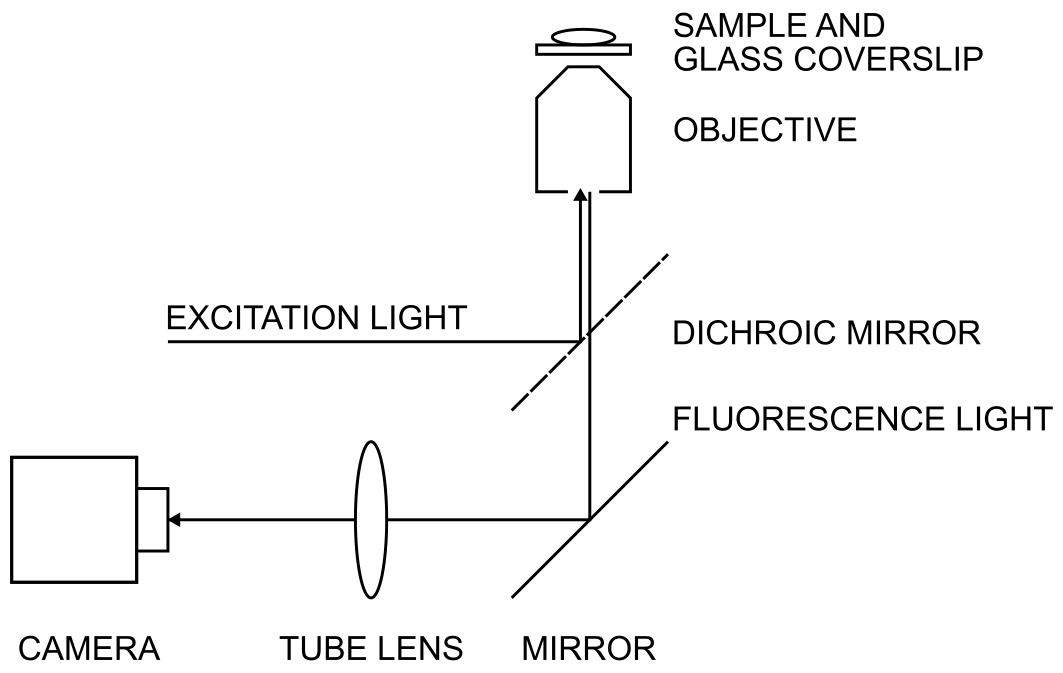
\includegraphics{epifluorescence-microscope.png}
    \caption{Principle components of an infinity corrected epifluorescence microscope.}
    \label{fig:epifluorescence-microscope}
\end{figure}

\chapter{Single Molecule Localization Microscopy}

\chapter{Fluorescence Photophysics}

\chapter{Localization Microscopy in Practice}

\begin{figure}[ht]
    \centering
    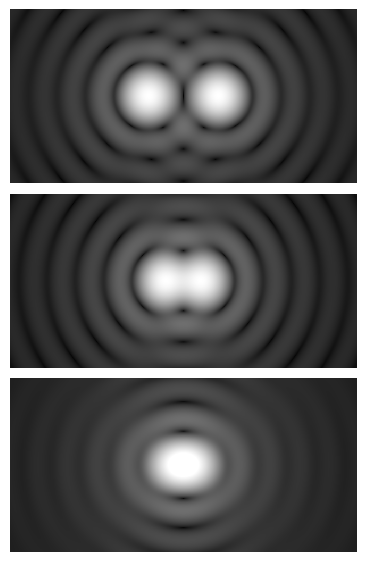
\includegraphics[width=0.75\textwidth]{Airy_disk_spacing_near_Rayleigh_criterion.png}
    \caption{Rayleigh criterion}
    \label{fig:rayleigh}
\end{figure}

\end{document}
